\documentclass[11pt,aspectratio=169]{beamer}

\usetheme{Madrid}
\usecolortheme{beaver}
\setbeamertemplate{navigation symbols}{}

\usepackage[utf8]{inputenc}
\usepackage[T1]{fontenc}
\usepackage{amsmath,amssymb}
\usepackage{booktabs}
\usepackage{listings}
\usepackage{xcolor}
\usepackage{tikz}
\usepackage{tcolorbox}
\tcbuselibrary{skins,breakable}

\definecolor{codebg}{RGB}{245,245,245}
\definecolor{codekw}{RGB}{0,0,180}
\lstdefinestyle{latexcode}{
  backgroundcolor=\color{codebg},
  basicstyle=\ttfamily\scriptsize,
  keywordstyle=\color{codekw}\bfseries,
  commentstyle=\color{gray},
  frame=single,
  rulecolor=\color{gray!40},
  breaklines=true,
  showstringspaces=false,
  xleftmargin=4pt,
  xrightmargin=4pt,
}
\lstset{style=latexcode}

\newtcolorbox{outputbox}{
  colback=white, colframe=black!65, boxrule=0.5pt, arc=1pt,
  left=8pt, right=8pt, top=5pt, bottom=4pt,
  title=\textsc{Compiled Output}, fonttitle=\bfseries\scriptsize,
  coltitle=white, colbacktitle=black!65
}
\newcommand{\whybox}[1]{%
  \vspace{2pt}
  {\scriptsize\raggedright\textcolor{red!55!black}{\textbf{Why \& What:}}~#1\par}
}

\newtcolorbox{exercisebox}{
  colback=orange!8, colframe=orange!70!black, boxrule=0.6pt,
  arc=2pt, left=6pt, right=6pt, top=4pt, bottom=4pt,
  title={Hands-on Exercise}, fonttitle=\bfseries, coltitle=white,
  colbacktitle=orange!70!black
}
\newtcolorbox{homeworkbox}{
  colback=blue!6, colframe=blue!50!black, boxrule=0.6pt,
  arc=2pt, left=6pt, right=6pt, top=4pt, bottom=4pt,
  title={Homework}, fonttitle=\bfseries, coltitle=white,
  colbacktitle=blue!50!black
}

\title[\texttt{\textbackslash begin} to \texttt{\textbackslash end}]{From \texttt{\textbackslash begin} to \texttt{\textbackslash end}}
\subtitle{The Complete LaTeX Guide \\[2pt] \normalsize Day 3 of 7: Tables, Figures \& Regression Output}
\author[A.\ Rahman]{Atikur Rahman}
\institute[White Globe Initiative]{White Globe Initiative}

\setbeamertemplate{footline}{
  \leavevmode
  \hbox{%
  \begin{beamercolorbox}[wd=.38\paperwidth,ht=2.5ex,dp=1.125ex,leftskip=1em]{author in head/foot}%
    \usebeamerfont{author in head/foot}White Globe Initiative
  \end{beamercolorbox}%
  \begin{beamercolorbox}[wd=.42\paperwidth,ht=2.5ex,dp=1.125ex,center]{title in head/foot}%
    \usebeamerfont{title in head/foot}From \texttt{\textbackslash begin} to \texttt{\textbackslash end} --- Day 3
  \end{beamercolorbox}%
  \begin{beamercolorbox}[wd=.20\paperwidth,ht=2.5ex,dp=1.125ex,right,rightskip=1em]{date in head/foot}%
    \usebeamerfont{date in head/foot}\insertframenumber{} / \inserttotalframenumber
  \end{beamercolorbox}}%
  \vskip0pt
}

\begin{document}

\begin{frame}[plain]
  \begin{center}
    \vspace{4pt}
    {\Huge\bfseries\usebeamercolor[fg]{title}From \texttt{\textbackslash begin} to \texttt{\textbackslash end}}\\[6pt]
    {\Large\itshape The Complete LaTeX Guide}\\[18pt]
    {\large\bfseries Day 3 of 7 --- Tables, Figures \& Regression Output}\\[22pt]
    \rule{0.7\textwidth}{0.4pt}\\[14pt]
    \begin{tabular}{rl}
      \textbf{Instructor:}       & Atikur Rahman \\[3pt]
      \textbf{Organized by:}     & White Globe Initiative \\[3pt]
      \textbf{Instructor Email:} & \texttt{atik@whiteglobeinitiative.org} \\[3pt]
      \textbf{General Contact:}  & \texttt{contact@whiteglobeinitiative.org} \\[3pt]
      \textbf{Format:}           & 7-Day Intensive Course \\[3pt]
      \textbf{Session:}          & Day 3 of 7 \\
    \end{tabular}\\[18pt]
    \rule{0.7\textwidth}{0.4pt}
  \end{center}
\end{frame}

\begin{frame}{Today's Agenda}
  \tableofcontents
\end{frame}

\section{Recap \& Today's Goal}

\begin{frame}{Quick Recap: Day 2}
  \small
  Yesterday: inline vs.\ display math, the \texttt{amsmath} package,
  subscripts/superscripts, Greek letters, operators, multi-line
  derivations with \texttt{align}, matrices, and equation labeling.
  \vspace{6pt}

  \textbf{Today's goal:} tables and figures are usually the hardest
  part for anyone switching from Word/Excel or Stata. Leave today with
  a repeatable workflow for turning regression output and charts into
  clean, journal-style tables and figures.
\end{frame}

\section{The tabular Environment}

\begin{frame}[fragile]{The Basics: tabular}
  \begin{lstlisting}
\begin{tabular}{lcc}
  Country & GDP Growth & Inflation \\
  Bangladesh & 6.0\% & 5.4\% \\
  India & 7.2\% & 5.1\% \\
\end{tabular}
  \end{lstlisting}
  \begin{outputbox}
    \small
    \begin{tabular}{lcc}
      Country & GDP Growth & Inflation \\
      Bangladesh & 6.0\% & 5.4\% \\
      India & 7.2\% & 5.1\% \\
    \end{tabular}
  \end{outputbox}
  \whybox{Column spec \texttt{\{lcc\}} sets alignment per column:
  \texttt{l} = left, \texttt{c} = center, \texttt{r} = right.
  \texttt{\&} separates columns, \texttt{\textbackslash\textbackslash}
  ends a row -- same grid logic as the matrices from Day 2. Notice
  there are \textbf{no lines} in the output: plain \texttt{tabular}
  draws no borders at all, which is why the next slide matters.}
\end{frame}

\section{booktabs: Publication-Quality Rules}

\begin{frame}[fragile]{booktabs: The Economics-Journal Look}
  \begin{lstlisting}
\usepackage{booktabs}

\begin{tabular}{lcc}
  \toprule
  Country & GDP Growth & Inflation \\
  \midrule
  Bangladesh & 6.0\% & 5.4\% \\
  \bottomrule
\end{tabular}
  \end{lstlisting}
  \begin{outputbox}
    \small
    \begin{tabular}{lcc}
      \toprule
      Country & GDP Growth & Inflation \\
      \midrule
      Bangladesh & 6.0\% & 5.4\% \\
      \bottomrule
    \end{tabular}
  \end{outputbox}
  \whybox{\texttt{\textbackslash toprule}, \texttt{\textbackslash
  midrule}, \texttt{\textbackslash bottomrule} add clean horizontal
  rules with no vertical lines -- this is the standard look in
  economics journals (AER, QJE, JPE all format tables this way). Never
  mix \texttt{\textbackslash hline} with booktabs rules in one table --
  the spacing is calibrated for one style or the other.}
\end{frame}

\section{multicolumn \& multirow}

\begin{frame}[fragile]{Grouped Headers with multicolumn}
  \vspace{-4pt}
  \begin{lstlisting}[basicstyle=\ttfamily\tiny,aboveskip=1pt,belowskip=1pt]
\begin{tabular}{lccc}
  \toprule
  & \multicolumn{3}{c}{Model} \\
  \cmidrule(lr){2-4}
  Variable & (1) & (2) & (3) \\
  \midrule
  Education & 0.08 & 0.07 & 0.07 \\
  \bottomrule
\end{tabular}
  \end{lstlisting}
  \begin{outputbox}
    \footnotesize
    \begin{tabular}{lccc}
      \toprule
      & \multicolumn{3}{c}{Model} \\
      \cmidrule(lr){2-4}
      Variable & (1) & (2) & (3) \\
      \midrule
      Education & 0.08 & 0.07 & 0.07 \\
      \bottomrule
    \end{tabular}
  \end{outputbox}
  \whybox{\texttt{\textbackslash multicolumn} merges 3 columns under
  one centered heading; \texttt{\textbackslash cmidrule(lr)\{2-4\}}
  draws a partial rule under just those columns -- the standard way to
  label ``(1)/(2)/(3)'' blocks. \texttt{multirow} does the same for
  merged \emph{rows}.}
\end{frame}

\section{A Complete Regression Table}

\begin{frame}{Putting It Together: A Regression Table}
  \footnotesize
  \begin{center}
  \begin{tabular}{lccc}
    \toprule
     & (1) & (2) & (3) \\
     & Baseline & +Controls & +Fixed Effects \\
    \midrule
    Education & 0.082*** & 0.075*** & 0.069*** \\
     & (0.011) & (0.010) & (0.012) \\
    Experience & & 0.021** & 0.019** \\
     & & (0.009) & (0.008) \\
    Constant & 8.21*** & 7.95*** & 8.02*** \\
     & (0.15) & (0.18) & (0.20) \\
    \midrule
    Observations & 1{,}204 & 1{,}204 & 1{,}204 \\
    $R^2$ & 0.14 & 0.19 & 0.23 \\
    \bottomrule
  \end{tabular}
  \end{center}
  \vspace{4pt}
  \whybox{Every tool on this slide comes from the last three: standard
  errors sit in parentheses \emph{below} each coefficient by leaving
  the variable-name cell blank on that row; significance stars
  (***~p$<$0.01, **~p$<$0.05) are just typed as literal text. This one
  table is \texttt{tabular} + \texttt{booktabs} + \texttt{multicolumn}
  and nothing else -- the exact structure of a real published
  regression table.}
\end{frame}

\section{Figures}

\begin{frame}[fragile]{The figure Environment}
  \begin{lstlisting}
\begin{figure}[htbp]
  \centering
  \includegraphics[width=0.6\textwidth]{gdp_growth.png}
  \caption{GDP growth rate, 2010--2024}
  \label{fig:gdp}
\end{figure}
  \end{lstlisting}
  \begin{outputbox}
    \centering
    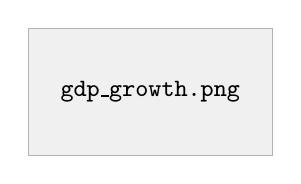
\begin{tikzpicture}[scale=0.62]
      \draw[fill=gray!12, draw=gray!60] (0,0) rectangle (5,2.6);
      \node at (2.5,1.3) {\small\texttt{gdp\_growth.png}};
    \end{tikzpicture}\\
    \footnotesize Figure 1: GDP growth rate, 2010--2024
  \end{outputbox}
  \whybox{\texttt{\textbackslash includegraphics} inserts an image
  file you've uploaded to your Overleaf project -- typically a chart
  exported from Stata (\texttt{graph export}), R, or Excel.
  \texttt{\textbackslash caption} and \texttt{\textbackslash label}
  work exactly as with tables: the caption is numbered automatically
  (``Figure 1'') and the label lets you reference it elsewhere with
  \texttt{\textbackslash ref\{fig:gdp\}}.}
\end{frame}

\section{Float Placement}

\begin{frame}[fragile]{Float Placement: Why Tables ``Wander''}
  \begin{lstlisting}
\begin{table}[htbp]
  ...
\end{table}
  \end{lstlisting}
  \whybox{\texttt{h} = here, \texttt{t} = top of page, \texttt{b} =
  bottom, \texttt{p} = a dedicated page of its own. \texttt{htbp} lets
  LaTeX choose the best fit among all four -- and it often
  \textbf{moves} your table to keep good page layout. This is normal:
  tables and figures are \textbf{floats}, not fixed text. Fighting
  placement aggressively (forcing \texttt{[H]} via the \texttt{float}
  package) usually looks worse than trusting the default algorithm.
  There is no single ``output'' to show here -- the point \emph{is}
  that the position is not fixed.}
\end{frame}

\section{Workflow: tablesgenerator.com}

\begin{frame}{Fast Workflow: Excel/Stata to LaTeX}
  \small
  \begin{enumerate}
    \item Copy your regression output or Excel range.
    \item Paste into \textbf{tablesgenerator.com} -- it renders a live preview as you paste.
    \item Choose the \textbf{booktabs} style in its formatting options.
    \item Export the generated \texttt{tabular} code and paste it into Overleaf.
    \item Hand-edit: add \texttt{\textbackslash caption}, \texttt{\textbackslash label}, and significance notes.
  \end{enumerate}
  \vspace{4pt}
  This is the standard shortcut used in practice -- nobody hand-types
  large tables from scratch.
\end{frame}

\section{Practice}

\begin{frame}{Hands-on Exercise}
  \begin{exercisebox}
    Take a small regression output table (from Stata, R, or a mocked-up
    dataset) and reproduce it in booktabs style:
    \begin{enumerate}
      \item Paste the data into tablesgenerator.com as a first pass.
      \item Bring the generated code into Overleaf.
      \item Hand-edit for a correct \texttt{\textbackslash caption} and \texttt{\textbackslash label}.
      \item Add a grouped header using \texttt{\textbackslash multicolumn} for at least two model columns.
    \end{enumerate}
  \end{exercisebox}
\end{frame}

\begin{frame}{Homework Before Day 4}
  \begin{homeworkbox}
    Insert all tables and figures from your running paper draft, with
    proper captions and labels for every one. If you don't yet have
    charts, mock up at least one placeholder figure with a caption.
  \end{homeworkbox}
  \vspace{10pt}
  \small\textbf{Resources for today:}
  \begin{itemize}\small
    \item Overleaf -- ``Tables'' / ``Positioning Images and Tables''
    \item Overleaf -- ``Lists of Tables and Figures''
    \item tablesgenerator.com
    \item Wikibooks LaTeX -- Tables and Floats chapters
  \end{itemize}
\end{frame}

\begin{frame}{Coming Up: Day 4}
  \Large
  \centering
  Citations \& Bibliography \\[6pt]
  \normalsize
  BibTeX, natbib, and building an author-year citation pipeline for
  your literature review.
\end{frame}

\begin{frame}[plain]
  \begin{center}
    \vspace{35pt}
    {\Large\bfseries Thank You}\\[10pt]
    {\large From \texttt{\textbackslash begin} to \texttt{\textbackslash end}: The Complete LaTeX Guide}\\[4pt]
    Day 3 of 7 --- Tables, Figures \& Regression Output\\[20pt]
    \rule{0.5\textwidth}{0.4pt}\\[10pt]
    Atikur Rahman \\
    White Globe Initiative \\[2pt]
    \texttt{atik@whiteglobeinitiative.org} \\
    \texttt{contact@whiteglobeinitiative.org}
  \end{center}
\end{frame}

\end{document}
